\documentclass{article}
\usepackage{tabularx}
\usepackage{amsmath}
\usepackage{graphicx}
\usepackage[top = 2cm, bottom = 2cm, right = 2cm, left = 2cm]{geometry}
\usepackage{cite}
\usepackage[final]{hyperref}
\usepackage{listings}
\hypersetup{
	colorlinks=true,
	linkcolor=blue,
	citecolor=blue,
	filecolor=magenta,
	urlcolor=blue         
}

\begin{document}

\title{Practicle 6\\Random with CUDA}
\date{06/02/19}
\maketitle

\begin{abstract}
	
\end{abstract}

\section{Microfacet models for material}
If you take a look on a material, like a metal for example, it seem perfectly flat, but, if you look very close to the surface you may see micro details. Like a light beam, each rays sent intersect the surface and are reflected or refracted. When a ray intersect a surface he lost energy. When a ray is sent between two object it will be reflected many time and lost a lot of energy. This part of the scene will be dark. This kind of shadow is called ambient occlusion and don't need light.

\begin{figure}[h]
	\centering
	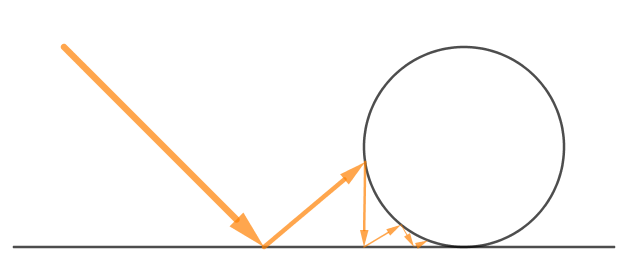
\includegraphics[scale=0.47]{figures/absorption.png}
	\caption{Absorption}
\end{figure}

For this practical we'll work on three different materials. We can define a material by a scatter function. The aim of this function is to evaluate the reflected or refracted ray from the initial ray. Because we want to use a stochastic methode to send ray we have to now how random works in CUDA.

\section{An other layout}
This section is optional. It's just to test an other way to organize pixel access on kernel. For the moment we read a pixel and we jump to the next one using the stride. Our rendering kernel will become very heavy so we need to use one thread per pixel. we'll divide our image into small image (8 pixels x 8 pixels). Create two variable in the host code for the number of blocks per grid and the number of threads per block.
\begin{lstlisting}
	dim3 blocks(width/8+1, height/8+1);
	dim3 threads(8, 8);
\end{lstlisting}
We can now run our kernel using this variable.

\begin{lstlisting}
	render<<<blocks, threads>>>(/*...*/);
\end{lstlisting}

Inside the kernel we can compute x and y in this way:
\begin{lstlisting}
	int x = threadIdx.x + blockIdx.x * blockDim.x;
	int y = threadIdx.y + blockIdx.y * blockDim.y;
	int index = y*width + x;
\end{lstlisting}
If you don't use a power of two for your image resolution, make sure the x and y values aren't greater than the width and the height.

\section{Generate random number}
To generate random number we need the cuRAND library. For that we should include curand\_kernel.h. This library provides an efficient generation of pseudorandom numbers. That means a sequence of numbers who have the same property as a truly random sequence. This sequence is generate by a deterministic algorithm.

\subsection{One random number}
If you need only one random number per pixel you can use the curand host library. Add curand.lib into your link dependencies and the include curand.h. For this section we'll generate number in the device and send the data to the host. On the host code create the generator:

\begin{lstlisting}
	curandGenerator_t generator;
	curandCreateGenerator(&generator, CURAND_RNG_PSEUDO_DEFAULT);
	curandSetPseudoRandomGeneratorSeed(generator, 4242ULL);
\end{lstlisting}

If needed more function are available here (https://docs.nvidia.com/cuda/curand/host-api-overview.html\#generator-types).\\
As usual allocate a buffer of float for each pixel on the host and device memory. We can now generate the number on the device using curandGenerateUniform for example.

\begin{lstlisting}
	curandGenerateUniform(generator, deviceFloatArray, width*height);
\end{lstlisting}

(Optional) If you need the buffer you can grab it from the device.
\begin{lstlisting}
	cudaMemcpy(hostFloatArray, deviceFloatArray,
		width*height*sizeof(float), cudaMemcpyDeviceToHost);
\end{lstlisting}

As the background clear color, write a kernel for drawing the random number. 

\begin{lstlisting}
	//...
	image[i] = Vector3(devData[index], devData[index], devData[index]);
	//...
\end{lstlisting}

You should get this kind of image. For information, noises like this one is part of a lot of algorithm for image generation.
\begin{figure}[h]
	\centering
	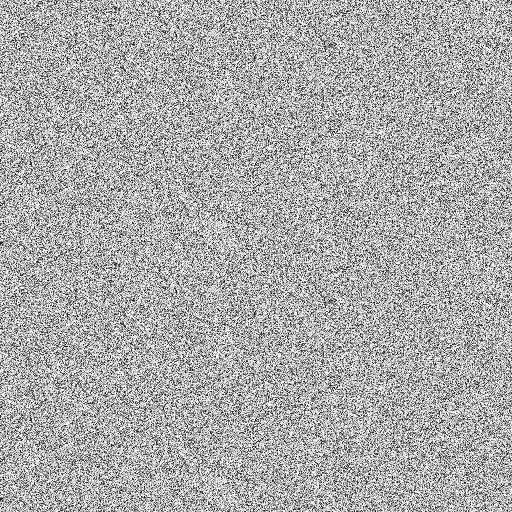
\includegraphics[scale=0.47]{figures/random.png}
	\caption{Uniform noise}
\end{figure}


\newpage
\subsection{Random sequence}
A pseudorandom sequence have to be initialize on a kernel. This operation can be very heavy so we will check carefully errors. First, we need a curandState per pixel. Use cudaMalloc to allocate one curandState per pixel on the device memory. Then run a new kernel named random\_initialization. In this kernel you have to call curand\_init.
 \begin{lstlisting}
	curand_init(seed, index, 0, &state[index]);
\end{lstlisting}
The seed is a kind of id for the pseudorandom sequence generation. If you use the same seed, you will have the same sequence. If you want different random number per pixel with the same seed we just have to define a subsequence (second parameter). The parameter three is the offset.\\
On your application, disable all kernels except this one and run you exe using cuda-memcheck. If errors is occurred, use the index as offset instead of subsequence. (There are some bugs with this library with CUDA 10 for the moment)
\begin{lstlisting}
	curand_init(seed, 0, index, &state[index]);
\end{lstlisting}
If it's good, reactivate your kernel.\\
Now, if you need random value, you just need to pass the curandState* buffer to your kernel and use the curand\_uniform function for pseudorandom uniform number.

\begin{lstlisting}
	float number = curand_uniform(&states[index])); // 0.f <= number <= 1.f
\end{lstlisting}

\newpage
\section{Diffuse material}
On your rendering kernel, call a device function named computeColor. On this function we'll compute the color for a ray sent. 

\begin{lstlisting}
	__device__
	Vector3 // The output color
		computeColor(
			const Ray& ray, // A ray sent
			Sphere** spheres, // The world
			unsigned int nbSphere,
			curandState* randomStates, // The buffer of states
			int nbRebound,
			const Vector3& backgroundColor);
\end{lstlisting}
On the first part of the function, compute the intersection with the ray and spheres. We'll use this struct for storing information.
\begin{lstlisting}
	struct HitInformation {
		bool hit_;
		float t_;
		Vector3 intersection_;
		Vector3 normal_;
	};
\end{lstlisting}
Your hit function can be simplify:
\begin{lstlisting}
	if (root0>0.001f && root0<hit.t_) {
		hit.hit_ = true;
		hit.t_ = root0;
		hit.intersection_ = ray.getOrigin()+ray.getDirection()*hit.t_;
		hit.normal_ = hit.intersection_-center_;
		hit.normal_.normalize();
		return true;
	}
\end{lstlisting}
If the ray send hit a sphere, you can compute recursively the scattered ray and the attenuation color. 
\begin{lstlisting}
	if (hit.hit_) {
		Ray scattered;
		Vector3 attenuation;
		if (nbRebound>0) {
			Ray scattered;
			Vector3 attenuation;
			//...
			return attenuation * computeColor(
				scattered,
				spheres,
				nbSphere,
				randomStates,
				--nbRebound,
				backgroundColor);
		} else {
			return Vector3(0.f, 0.f, 0.f);
		}
	} else {
		return backgroundColor;
	}
\end{lstlisting}
For a diffuse material, we use a simplify model of the Lambertian reflectance. Each rays will be reflected randomly while they hit a sphere.

\begin{lstlisting}
	Vector3 target = hit.intersection_ + hit.normal_ + randomSphereUnitVector(states);
	rayScattered = Ray(hit.intersection_, (target-hit.intersection_));
	attenuation = SphereColor_;
\end{lstlisting}

For generate a vector into the unit sphere you just have to generate a vector with random value minus $(0.5, 0.5, 0.5)$ and normalize it.\\
At this point you can run your recursive function 10 times but, not 50 time because you call stack is to small. You can modify the size of your call stack using cudaDeviceSetLimit(cudaLimitStackSize, value). The problem is, if you increase your call stack, you reduce the number of register for the computation. The best way is to make an iterative algorithm.

\begin{lstlisting}
	Ray r = ray;
	Vector3 cur_attenuation = Vector3(1.f, 1.f, 1.f);
	for (int i = 0; i<nbRebound; ++i) {
		//...
		if (hit.hit_) {
			Ray scattered;
			Vector3 attenuation;
			Vector3 target = hit.intersection_ + hit.normal_ + randomSphereUnitVector(states);
			rayScattered = Ray(hit.intersection_, (target-hit.intersection_));
			attenuation = SphereColor_;
		} else {
			return cur_attenuation*backgroundColor;
		}
	}
	return Vector3(0.f, 0.f, 0.f);
\end{lstlisting}
You may have a similar results:
\begin{figure}[h]
	\centering
	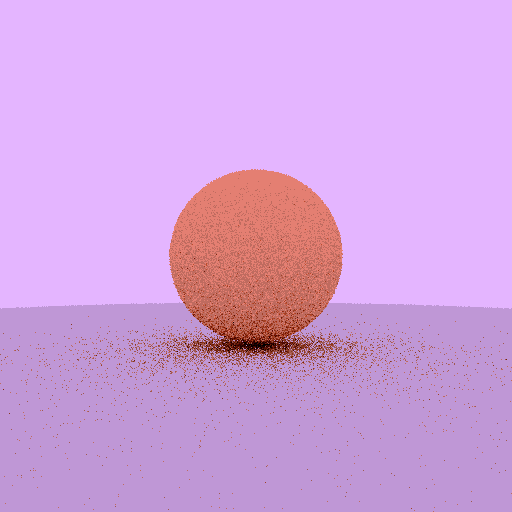
\includegraphics[scale=0.47]{figures/oneRay.png}
	\caption{Ambiante Occlusion with one ray}
\end{figure}

\subsection{TDR}
The Timeout Detection \& Recovery (TDR) is the Windows's feature to detect response problems from the graphics card. If your application run a kernel for more than two seconds, Windows reset the card. The aim of this feature is to avoid system freeze when a segmentation fault or an infinite loop appear on kernel.\\

\subsection{multiple ray per pixel}
To increase the result, we need to send more than one ray per pixel. To avoid a TDR we'll run the rendering kernel 100 times instead of add a loop inside the kernel.
\begin{lstlisting}
	for (int i = 0; i<nbRayPerPixel; ++i) {
		rayTraceGPU<<<blocks, threads>>>(/*...*/);
	}
\end{lstlisting}

Currently I use my image for storing the result. Now I need to use the image to store intermediate result. So, I have to clear my image with black value. After that, each call of the kernel has to accumulate the result into image.

\begin{figure}[h]
	\centering
	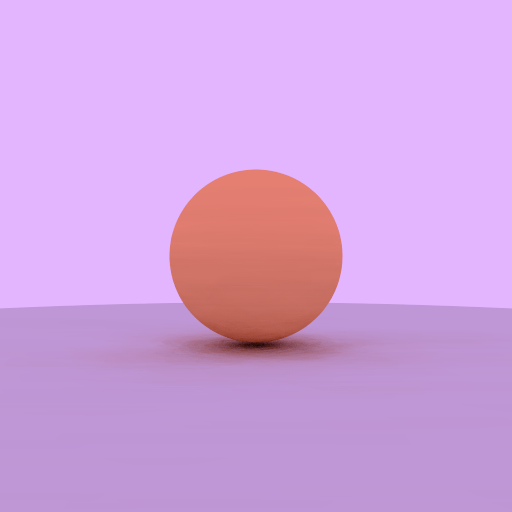
\includegraphics[scale=0.47]{figures/result.png}
	\caption{Ambiante Occlusion with 100 rays}
\end{figure}

All computations we did are done on a linear space. This space is perfect for computation but, wrong for our perception. We need to apply a gamma correction. The common correction is the sRGB curve (gamma 2.2). But, for this exercice we just need a gamma 2 correction. On the writeBufferAsBMP compute the sqrt of the color before the cast of the color.
\begin{lstlisting}
	unsigned char pixelc[3]{
		unsigned char(255.99f*sqrt(buffer[x+w*y].b())),
		unsigned char(255.99f*sqrt(buffer[x+w*y].g())),
		unsigned char(255.99f*sqrt(buffer[x+w*y].r())),
	};
\end{lstlisting}

\end{document}